\documentclass[10pt]{beamer}
\usepackage{graphicx}
\usepackage{listings}
\usepackage{multicol}
%\usepackage{showframe}

\mode<presentation>{
    \usetheme{redhat}
%    \setbeameroption{show notes on second screen=right}
}

% https://github.com/josephwright/beamer/issues/337
%\makeatletter
%\def\beamer@framenotesbegin{%
%  \usebeamercolor[fg]{normal text}%
%  \gdef\beamer@noteitems{}%
%  \gdef\beamer@notes{}%
%}
%\makeatother

\setcounter{tocdepth}{2}
\newcommand{\autotitle}{
    \frametitle{
        \secname
        \ifx \insertsubsection \empty \else { / \MakeLowercase{\subsecname}} \fi
    }
}

\title{\texttt{ci-operator}}
\subtitle{(not an operator)}

\author{Bruno Barcarol Guimarães}
\institute[]{Red Hat}
\date{2022-06-28}

\begin{document}

\begin{frame}
    \titlepage
\end{frame}

\begin{frame}
    \frametitle{Overview}
    \tableofcontents
\end{frame}

\section{History}
\subsection{\texttt{ci-tools}}

\defverbatim\tmpverb{
    \scriptsize
    \begin{verbatim}
$ git log --format='%ad %an %s' --date=format-local:%Y-%m-%d | tail -3
2018-01-31 Steve Kuznetsov Initial implementation of the ci-operator code
2018-01-31 Steve Kuznetsov Initialize vendor directory with Glide
2018-01-31 Steve Kuznetsov Initialize .gitignore
    \end{verbatim} %$
}

\begin{frame}
    \autotitle
    \footnotesize
    \only<1>{\url{https://github.com/openshift/ci-tools/graphs/contributors}}
    \vfill
    \centering
    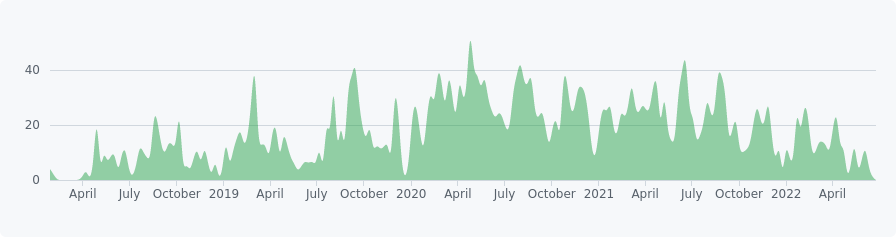
\includegraphics[width=\linewidth]{img/contributors.png}
    \only<1>{\tmpverb}
    \vfill
    \includegraphics<2>[scale=.4]{img/contributors_bbguimaraes.png}
    \note<1>{
        Here is the contributor graph for \texttt{ci-tools}, going back to 2018
        --- the small mount at the beginning is 31 Jan.  You can see the
        "initial implementation of […] \texttt{ci-operator}" in the \texttt{git}
        log.

        None of the original authors remains in the team (in fact, only one
        remains in the company), but the code lives on.
    }
    \note<2>{
        I am the chief code deleter \texttt{=)} (these numbers make little sense
        since we include the \texttt{vendor} directory in the repository)

        I was involved but not directly participating in the beginning, back
        then we were part of the "CI/CD" team and I worked on both sides of the
        slash.  The first thing I remember working on was the implementation of
        the \texttt{--target} argument, although my version is not the one in
        the repository (development was chaotic at the time).
    }
\end{frame}

\begin{frame}[fragile]
    \autotitle
    \tiny
    \begin{verbatim}
$ git log --format='%ad %an %s' --date=format-local:%Y-%m-%d --graph 78af6eb7c
* 2019-06-13 Bruno Barcarol Guimarães Merge Makefiles
*   2019-06-13 Bruno Barcarol Guimarães Merge ci-operator-prowgen
|\
…
| * 2018-08-23 Steve Kuznetsov Add an OWNERS file
| * 2018-08-23 Steve Kuznetsov Reorganize code, add Makefile
| * 2018-08-23 Steve Kuznetsov Copy content from openshift/release
*   2019-06-13 Bruno Barcarol Guimarães Merge ci-operator
|\
…
| * 2018-04-06 Clayton Coleman Add .gitignore for binary
| * 2018-02-09 Steve Kuznetsov Refactor StepLink to be functional
| * 2018-02-08 Steve Kuznetsov Add the release tagging step
| * 2018-02-02 Steve Kuznetsov Add a dry-run mode to the entrypoint
| * 2018-01-31 Steve Kuznetsov Initial implementation of the ci-operator code
| * 2018-01-31 Steve Kuznetsov Initialize vendor directory with Glide
| * 2018-01-31 Steve Kuznetsov Initialize .gitignore
* 2019-06-13 Bruno Barcarol Guimarães Initial commit
    \end{verbatim} %$
    \note{
        If you've ever looked at the repository's history, you might have seen
        it is a bit strange.  There are commits named "merge
        \texttt{Makefile}s", "merge \texttt{ci-operator-prowgen}", and "merge
        \texttt{ci-operator}", followed by forks in the history (n.b.: not
        branches) with their own histories and initial commits, and finally an
        "initial commit" a year and a half \emph{later}.
    }
\end{frame}

\begin{frame}
    \autotitle
    \small \let\small\footnotesize
    \begin{itemize}
        \item \url{https://github.com/openshift/ci-tools.git}
        \begin{itemize}
            \item \url{https://github.com/openshift/ci-operator.git}
            \item \url{https://github.com/openshift/ci-operator-prowgen.git}
            \item \ldots
        \end{itemize}
    \end{itemize}
    \note{
        This is because it started its life as multiple separate repositories
        that were later joined into what is now \texttt{ci-tools}.  Its
        precursors can still be found in Github and are still occasionally of
        historical significance (pull requests and issues are still there).
    }
\end{frame}

\begin{frame}[fragile]
    \autotitle
    \tiny
    \begin{verbatim}
$ git log --format=%ad --date=format-local:'%a %u' --author 'Bruno Barcarol Guimarães' \
    | sort | uniq -c | sort -nk 3,3 \
    | gnuplot …


  140 +--------------------------------------------------------------------+
      |           +          +           +         126          +          |
      |                                          *******                   |
  120 |-+                               112      *     *                 +-|
      |                               ******     *     *                   |
      |                     101       *    *     *     *                   |
  100 |-+                 *******     *    *     *     *                 +-|
      |                   *     *     *    *     *     *                   |
      |                   *     *     *    *     *     *       76          |
   80 |-+        71       *     *     *    *     *     *     ******      +-|
      |        ******     *     *     *    *     *     *     *    *        |
   60 |-+      *    *     *     *     *    *     *     *     *    *      +-|
      |        *    *     *     *     *    *     *     *     *    *        |
      |        *    *     *     *     *    *     *     *     *    *        |
   40 |-+      *    *     *     *     *    *     *     *     *    *      +-|
      |        *    *     *     *     *    *     *     *     *    *        |
      |        *    *     *     *     *    *     *     *     *    *        |
   20 |-+      *    *     *     *     *    *     *     *     *    *      +-|
      |        *    *     *     *     *    *     *     *     *    *        |
      |        *  + *     *  +  *     *  + *     *  +  *     *  + *        |
    0 +--------------------------------------------------------------------+
                 Mon        Tue         Wed        Thu         Fri
    \end{verbatim} %$
    \note{
        Other things you find when excavating through \texttt{git} logs: back
        then, development was \emph{very} chaotic, and Saturday/Sunday pushes
        were not uncommon.
    }
\end{frame}

\begin{frame}[fragile]
    \autotitle
    \tiny
    \begin{verbatim}
$ git log --format=%ad --date=format-local:'%a %u' --author 'Clayton Coleman' \
    | sort | uniq -c | sort -nk 3,3 \
    | gnuplot …


  60 +---------------------------------------------------------------------+
     |        +        +      53        +        +        +       +        |
     |                       *****                                         |
  50 |-+                     *   *                                       +-|
     |                       *   *              44                         |
     |                       *   *             *****                       |
     |                       *   *             *   *                       |
  40 |-+     35              *   *     37      *   *                     +-|
     |      *****     33     *   *    *****    *   *     34                |
     |      *   *   ******   *   *    *   *    *   *   ******              |
  30 |-+    *   *   *    *   *   *    *   *    *   *   *    *            +-|
     |      *   *   *    *   *   *    *   *    *   *   *    *              |
     |      *   *   *    *   *   *    *   *    *   *   *    *              |
  20 |-+    *   *   *    *   *   *    *   *    *   *   *    *    18      +-|
     |      *   *   *    *   *   *    *   *    *   *   *    *   *****      |
     |      *   *   *    *   *   *    *   *    *   *   *    *   *   *      |
     |      *   *   *    *   *   *    *   *    *   *   *    *   *   *      |
  10 |-+    *   *   *    *   *   *    *   *    *   *   *    *   *   *    +-|
     |      *   *   *    *   *   *    *   *    *   *   *    *   *   *      |
     |      * + *   *  + *   * + *    * + *    * + *   *  + *   * + *      |
   0 +---------------------------------------------------------------------+
             Mon      Tue     Wed      Thu      Fri      Sat     Sun
    \end{verbatim} %$
\end{frame}

\section{Motivation}
\begin{frame}
    \autotitle
    \begin{center}
        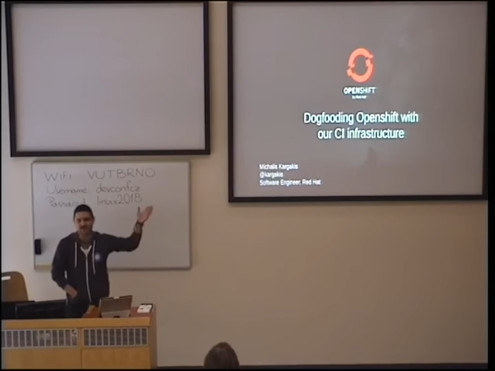
\includegraphics[scale=.4]{img/pres_2018.jpg} \\
        \textit{Dogfooding Openshift with our CI infrastructure}, \\
        Michalis Kargakis (2018-01-27) \\
        \url{https://www.youtube.com/watch?v=rLLEjodflYw}
    \end{center}
    \note{
        Continuing with the historical theme, but moving on to motivation, there
        is a presentation by Michalis which was posted in our chat recently.  It
        is contemporaneous --- n.b.: four days before the beginning of the
        \texttt{ci-operator} repository/history --- and goes through many of the
        problems the CI system at the time had.
    }
\end{frame}

\subsection{Past}

\begin{frame}
    \autotitle
    \begin{itemize}
        \item
            Jenkins \only<2>{(R.I.P.)}
            \begin{itemize}
                \item<2> Ruby (OpenShift v2), Python, Bash, \ldots
                \item<2> \emph{slow}
                \item<2> unmaintained
                \item<2> \emph{unmaintainable}
            \end{itemize}
        \item<2>
            Kubernetes
            \begin{itemize}
                \item \url{https://github.com/kubernetes/test-infra.git}
                \item Prow
            \end{itemize}
        \item<2>
            OpenShift
            \begin{itemize}
                \item \texttt{ImageStream}s
                \item \texttt{Build}s
                \item multi-tenancy
                \item \ldots
            \end{itemize}
    \end{itemize}
    \note{
        They can be summarized mostly with one word.

        The CI "system" was a mixture of Ruby (as was OpenShift v2), Python, and
        Bash scripts, used a very inefficient model on top of that, and was
        mostly unmaintained and unmaintainable.

        Meanwhile, Kubernetes (our upstream project) had \texttt{test-infra} and
        Prow: a CI system which used the platform itself and a language and
        concepts that were familiar to OpenShift developers.

        OpenShift also had many unique features which could be used to extend
        the upstream system (at the time, many were later contributed upstream,
        although a unique set still remains).

        So we decided to adopt Prow and integrate it into our product.
    }
\end{frame}

\subsection{Prow}

\begin{frame}[fragile]
    \autotitle
    \footnotesize
    \url{https://github.com/kubernetes/test-infra/blob/master/prow/life_of_a_prow_job.md}
    \scriptsize
    \begin{verbatim}
apiVersion: prow.k8s.io/v1
kind: ProwJob
metadata:
  name: 32456927-35d9-11e7-8d95-0a580a6c1504
spec:
  job: pull-test-infra-bazel
  decorate: true
  pod_spec:
    containers:
    - image: gcr.io/k8s-staging-test-infra/bazelbuild:latest-test-infra
  refs:
    base_ref: master
    base_sha: 064678510782db5b382df478bb374aaa32e577ea
    org: kubernetes
    pulls:
    - author: ixdy
      number: 2716
      sha: dc32ccc9ea3672ccc523b7cbaa8b00360b4183cd
    repo: test-infra
  type: presubmit
    \end{verbatim}
    \note{
        In Prow, the unit of work is the \texttt{ProwJob}: a native Kubernetes
        object which links the information from the repository (repository,
        revision, pull request, etc.) to the work that must be done in the build
        cluster (in the form of a \texttt{Pod} spec).
    }
\end{frame}

\begin{frame}[fragile]
    \autotitle
    \scriptsize
    \url{https://github.com/openshift/release/blob/master/ci-operator/jobs/openshift/ci-tools/openshift-ci-tools-master-presubmits.yaml}
    \begin{verbatim}
presubmits:
  openshift/ci-tools:
  - branches:
    - ^master$
    - ^master-
    cluster: build04
    labels:
      ci.openshift.io/generator: prowgen
      pj-rehearse.openshift.io/can-be-rehearsed: "true"
    name: pull-ci-openshift-ci-tools-master-unit
    spec:
      containers:
      - args:
        - --gcs-upload-secret=/secrets/gcs/service-account.json
        - --image-import-pull-secret=/etc/pull-secret/.dockerconfigjson
        - --report-credentials-file=/etc/report/credentials
        - --target=unit
        command:
        - ci-operator
        image: ci-operator:latest
    \end{verbatim} %$
    \note{
        A Prow job has to be registered before it can be executed.  We do that
        using files under \texttt{ci-operator/jobs} in the
        \texttt{openshift/release} repository.  Note that this is extremely
        anachronistic, almost nothing shown here existed at the time:
        \begin{itemize}
            \setlength\itemsep{-0.25em}
            \item there was only a single cluster
            \item there was no \texttt{prowgen}
            \item there was no \texttt{rehearse}
            \item artifact upload was done differently
            \item images were not imported from other clusters
            \item there was no results server
        \end{itemize}
        However, we do not want every user to have to build their CI pipeline
        from zero…
    }
\end{frame}

\begin{frame}[fragile]
    \autotitle
    \footnotesize
    \url{https://github.com/openshift/release/blob/master/ci-operator/config/openshift/ci-tools/openshift-ci-tools-master.yaml}
    \scriptsize
    \begin{multicols}{2}
    \begin{verbatim}
base_images:
  os:
    name: centos
    namespace: origin
    tag: stream8
binary_build_commands: >
  make production-install
build_root:
  from_repository: true
  use_build_cache: true
images:
- context_dir: >
    images/ci-operator/
  from: os
  inputs:
    bin:
      paths:
      - destination_dir: .
        source_path: >
          /go/bin/ci-operator
  to: ci-operator
  \end{verbatim}
  \columnbreak
  \begin{verbatim}
promotion:
  namespace: ci
  tag: latest
test_binary_build_commands: >
  make race-install
tests:
- as: unit
  commands: make test
  container:
    from: src
- as: e2e
  steps:
    test:
    - as: e2e
      commands: make e2e
      from: test-bin
    \end{verbatim} %$
    \end{multicols}
    \note{
        The \texttt{ci-operator} configuration file is a standard description of
        the CI pipe\-line for a given repository.  This is the configuration
        used in \texttt{ci-tools}.  It simpler because we are not an OpenShift
        component, but otherwise demonstrates the major concepts:
        \begin{itemize}
            \item input images
            \item image builds
            \item unit/E2E tests
            \item image promotion
        \end{itemize}
    }
\end{frame}

\section{Architecture}
\subsection{Overview}
\begin{frame}
    \autotitle
    \begin{itemize}
        \item
            \url{https://docs.ci.openshift.org}
            \begin{itemize}
                \item \href
                    {https://docs.ci.openshift.org/docs/architecture/ci-operator/}
                    {/docs/architecture/ci-operator}
                \item \href
                    {https://docs.ci.openshift.org/docs/internals/}
                    {/docs/internals}
                \item \href
                    {https://docs.ci.openshift.org/docs/internals/steps/}
                    {/docs/internals/steps}
            \end{itemize}
        \item
            \url{https://github.com/openshift/ci-docs/pulls}
            \begin{itemize}
                \item \href
                    {https://github.com/openshift/ci-docs/pull/233}
                    {\#233}
                \item \href
                    {https://github.com/openshift/ci-docs/pull/235}
                    {\#235}
                \item \href
                    {https://github.com/openshift/ci-docs/pull/266}
                    {\#266}
            \end{itemize}
    \end{itemize}
    \note{
        We have a few architectural descriptions of \texttt{ci-operator} and
        \texttt{ci-tools} in general.  The \texttt{architecture/ci-operator}
        page is meant for users but, since they are also developers, goes into
        fairly technical detail.  The \texttt{…-internals} page is meant for
        internal use and has abundant references to source code.

        Documenting (and understanding in the first place) is an ongoing effort,
        and there are several work-in-progress documents you can also consult.
    }
\end{frame}

\begin{frame}
    \autotitle
    \begin{center}
        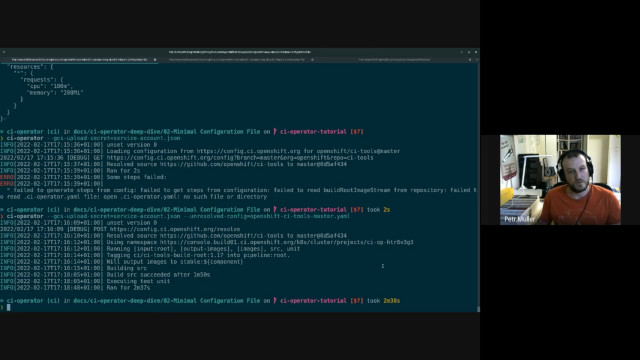
\includegraphics[scale=.4]{img/prev.jpg} \\
        \textit{Shift Week Knowledge Sharing}, Petr Muller (2022-02-17) \\
        \scriptsize
        \url{https://drive.google.com/file/d/1ye_Xim2oV4iJaQtBQrDUjre3vwDvZKDT/}
    \end{center}
    \note{
        I am going to take a different route than I normally would because we've
        already had a very good presentation by Petr in a previous knowledge
        sharing session.  It was remarkably similar to what I had in mind for a
        \texttt{ci-operator} introduction, and formed part of the basis for the
        development of \url{https://github.com/openshift/ci-docs/pull/235}.

        Instead, here we're going the opposite way, with an abstract
        architecture overview.
    }
\end{frame}

\begin{frame}
    \autotitle
    \begin{multicols}{2}
        \begin{itemize}
            \item
                Inputs
                \begin{itemize}
                    \item repository / \texttt{git} revision(s)
                    \item command-line arguments
                    \item configuration
                \end{itemize}
        \end{itemize}
        \begin{itemize}
            \item
                Outputs
                \begin{itemize}
                    \item test results
                    \item images
                \end{itemize}
        \end{itemize}
        \columnbreak
        \begin{itemize}
            \item<2>
                Implementation
                \begin{itemize}
                    \item build cluster/node
                    \item temporary namespace
                    \item image pipeline
                    \item test types
                    \item cloud providers
                    \item remote storage
                    \item image promotion
                \end{itemize}
        \end{itemize}
    \end{multicols}
    \note{
        Conceptually, the work done by \texttt{ci-operator} is relatively
        simple: it receives a list of source code references, command-line
        arguments, and a configuration file as input and produces test results
        and container images as output.  The devil is, as always, in the
        details.
    }
\end{frame}

\begin{frame}
    \autotitle
    \begin{quote}
        \texttt{ci-operator} is at its core a task scheduling program. The input
        configuration is processed and used to build a task graph, which is then
        executed until completion, failure, or interruption. Thus, the execution
        flow of \texttt{ci-operator} can be divided in these major phases:
        \begin{itemize}
            \item input processing
            \item task graph creation
            \item task graph execution
            \item cleanup
        \end{itemize}
    \end{quote}
    \note{
        This introduction from the "internals" documentation describes exactly
        what is needed to understand how \texttt{ci-operator} works.  The main
        data structure is the \textit{step graph}.
    }
\end{frame}

\begin{frame}[fragile]
    \autotitle
    \begin{verbatim}
$ ci-operator \
    --unresolved-config ci-tools-master.yaml \
    --print-graph \
    --target unit --target e2e
…
src [input:root]
test-bin src
unit src
e2e test-bin
…
    \end{verbatim} %$
    \url{https://pkg.go.dev/golang.org/x/tools/cmd/digraph}
    \note{
        There is an obscure flag which can be used to display the graph.  The
        output is meant to be used with the (equaly obscure) \texttt{digraph}
        Golang \href{https://pkg.go.dev/golang.org/x/tools/cmd/digraph}{tool}.
        Each line contains a step in the first column and its dependencies as
        subsequent columns.

        \textit{Note: some of the functionality described here (e.g. displaying
        a sub-graph with \texttt{--target}) is not yet in \texttt{master}.}
    }
\end{frame}

\begin{frame}[fragile]
    \autotitle
    \begin{verbatim}
$ ci-operator \
    --unresolved-config ci-tools-master.yaml \
    --print-graph \
    --target unit --target e2e \
    | hack/ci-operator/graphviz.pl -T png \
    > out.png
    \end{verbatim} %$
    \begin{center}
        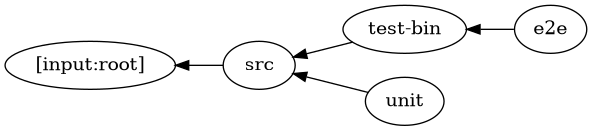
\includegraphics[scale=0.5]{img/graph.png}
        (requirement $\leftarrow$ dependent)
    \end{center}
    \note{
        With a bit of magic (a.k.a. Perl), it can be translated to the DOT
        language and visualized.
    }
\end{frame}

\begin{frame}
    \autotitle
    \begin{center}
        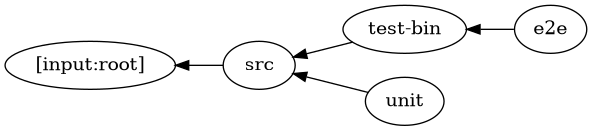
\includegraphics[scale=0.5]{img/graph.png}
    \end{center}
    \setlength\linewidth{40em}
    \setlength\columnsep{0cm}
    \begin{multicols}{2}
        \begin{itemize}
            \item import \texttt{root} image
                \begin{itemize}
                    \item \texttt{build\_root}
                    \item special name: \texttt{[input:…]}
                \end{itemize}
            \item build \texttt{src} image
                \begin{itemize}
                    \item
                        explicit requirement of \texttt{unit}, implicit
                        requirement of \texttt{test-bin}
                \end{itemize}
            \item build \texttt{test-bin} image
                \begin{itemize}
                    \item \texttt{test\_binary\_build\_commands}
                    \item
                        requested by \texttt{from:} \texttt{test-bin} in
                        \texttt{e2e}
                \end{itemize}
            \columnbreak
            \item execute \texttt{unit} test
                \begin{itemize}
                    \item \texttt{--target}
                \end{itemize}
            \item execute \texttt{e2e} test
                \begin{itemize}
                    \item \texttt{--target}
                \end{itemize}
        \end{itemize}
    \end{multicols}
\end{frame}

\begin{frame}[fragile]
    \autotitle
    \begin{verbatim}
… --target unit --target e2e --target ci-operator …
    \end{verbatim}
    \begin{center}
        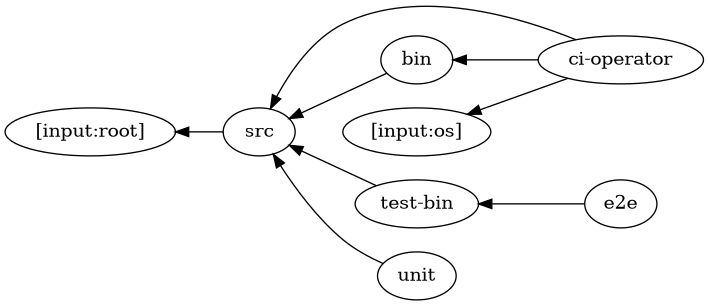
\includegraphics[scale=0.4]{img/graph_plus.png}
    \end{center}
    \note{
        If we add the \texttt{ci-operator} target to the graph (an image build),
        we can see the effect in the resulting graph:
        \begin{itemize}
            \item the previous graph is unchanged at the bottom
            \item the \texttt{ci-operator} node is added, unsurprisingly
            \item it uses an input image (\texttt{base\_images}) as a base
            \item
                it also uses the \texttt{bin} image as a base, which in turn is
                built from the \texttt{src} image
        \end{itemize}
    }
\end{frame}

\begin{frame}[fragile]
    \autotitle
    \footnotesize
    \begin{verbatim}
                                        0             0
INFO[2022-06-27T10:46:10Z] Running [input:root], [input:os], \
    src, bin, test-bin, ci-operator, unit, e2e
     1    2      2           3         2    3
    \end{verbatim}
    \begin{center}
        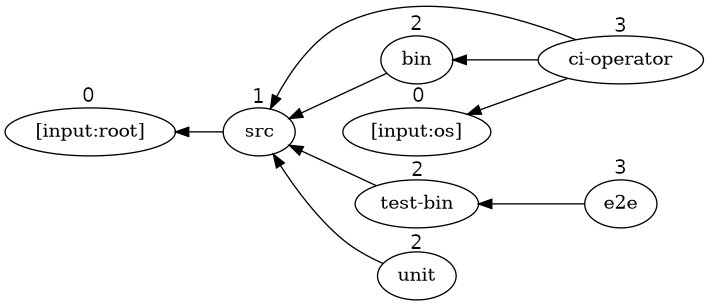
\includegraphics[scale=0.4]{img/graph_order.png}
    \end{center}
    \note{
        This graph is what the line in the \texttt{ci-operator} output which
        contains "Running" followed by a sequence of names represents: it is a
        topological order of the graph, i.e. a one-dimensional projection of the
        sequence(s) of steps to be performed.

        As described previously, these are all executed in parallel as much as
        possible, with dependent steps starting as soon as their requirements
        are satisfied.  This means this linearized version is only one of the
        possible total orders, as the dependency between steps is only a partial
        order.

        This visualization assigns a number to each node according to its
        "maximum depth" starting from the roots, giving an idea of which steps
        can be executed in parallel.
    }
\end{frame}

\begin{frame}[fragile]
    \autotitle
    \url{https://docs.ci.openshift.org/docs/internals/steps/#step-types}
    \vspace{1em}
    \begin{itemize}
        \item build steps
        \item release steps
        \item (optional) operator steps
        \item auxiliary steps
        \item test steps
        \item output steps
    \end{itemize}
    \note{
        Mastering \texttt{ci-operator} is in some sense learning the purpose and
        implementation of each type of step.  The "internals" page has sections
        for each category, with individual sub-sections for each and every step
        type.
    }
\end{frame}

\begin{frame}[fragile]
    \autotitle
    \href
        {https://github.com/openshift/ci-tools/blob/master/pkg/api/graph.go}
        {pkg/api/graph.go} (simplified)
    \begin{verbatim}
type Step interface {
    Name() string
    Description() string
    Requires() []StepLink
    Creates() []StepLink
    Inputs() (InputDefinition, error)
    Run(ctx context.Context) error
}

type StepNode struct {
    Step     Step
    Children []*StepNode
}
    \end{verbatim}
    \note{
        You can imagine what the execution code look like from that description,
        but here is a simplified version of it.  This is the step interface and
        the graph structure.
    }
\end{frame}

\begin{frame}[fragile]
    \autotitle
    \begin{verbatim}
// StepGraph is a DAG of steps referenced by
// its roots
type StepGraph []*StepNode

// OrderedStepList is a topologically-ordered
// sequence of steps.  Edges are determined
// based on the Creates/Requires methods.
type OrderedStepList []*StepNode
    \end{verbatim}
    \note{
        We have many types in \texttt{pkg/api/graph} which are all just slices
        of \texttt{StepNode} (\texttt{StepGraph}, \texttt{OrderedStepList},
        etc.).  Each is a separate type for semantic reasons.
    }
\end{frame}

\begin{frame}[fragile]
    \autotitle
    \scriptsize
    \begin{verbatim}
// TopologicalSort validates nodes form a DAG and orders them
// topologically.
func (g StepGraph) TopologicalSort() (OrderedStepList, []error) {
    …
    var waiting []*StepNode
    …
}
    \end{verbatim}
    \note{
        Here is a nice example with multiple types which are all the same
        underlying structure.
    }
\end{frame}

\begin{frame}[fragile]
    \autotitle
    \href
        {https://github.com/openshift/ci-tools/blob/master/pkg/steps/run.go}
        {pkg/steps/run.go} (simplified)
    \footnotesize
    \begin{verbatim}
func Run(graph api.StepGraph) {
    var seen []api.StepLink
    results := make(chan *api.StepNode)
    for _, root := range graph {
        go runStep(root, results)
    }
    for out := range results {
        seen = append(seen, out.Step.Creates()...)
        for _, child := range out.node.Children {
            if api.HasAllLinks(child.Step.Requires(), seen) {
                go runStep(child, results)
            }
        }
    }
}
    \end{verbatim}
    \note{
        And finally, the code which executes all steps in the graph.
    }
\end{frame}

\begin{frame}
    \autotitle
    \begin{center}
        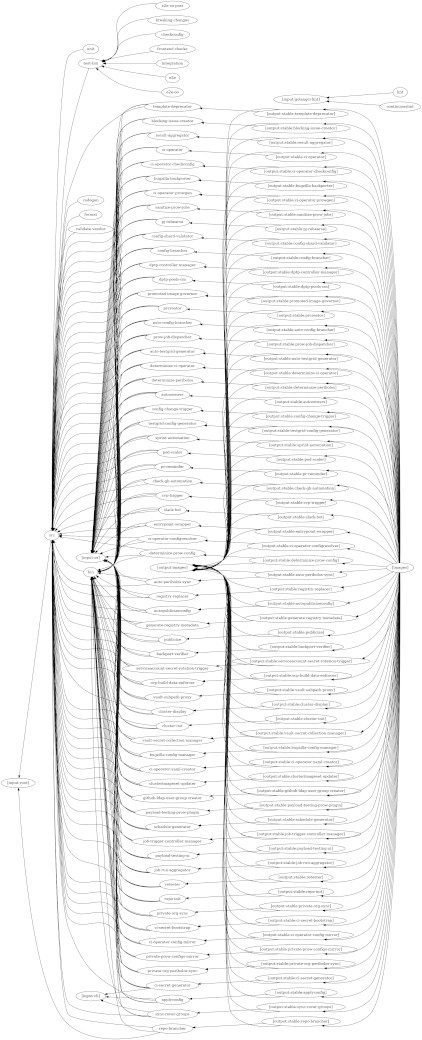
\includegraphics[height=20em]{img/ci-tools3.jpg}
    \end{center}
    \note{
        Of course, reality is \emph{much} more complicated… (this is the actual
        graph for \texttt{ci-tools}, which is still a long way from being as
        complicated as it can be)
    }
\end{frame}

\subsection{Initialization}
\begin{frame}[fragile]
    \autotitle
    \href
        {https://github.com/openshift/ci-tools/blob/master/cmd/ci-operator/main.go}
        {cmd/ci-operator/main.go}
    \footnotesize
    \begin{verbatim}
steps, postSteps, err := defaults.FromConfig(
    ctx, o.configSpec, &o.graphConfig, o.jobSpec,
    o.templates, o.writeParams, o.promote, o.clusterConfig,
    leaseClient, o.targets.values, o.cloneAuthConfig,
    o.pullSecret, o.pushSecret, o.censor, o.hiveKubeconfig,
    o.consoleHost, o.nodeName)
    \end{verbatim}
    \note{
        Moving on to what actually happens when \texttt{ci-operator} is
        executed, we start with this gigantic function call to turn all input
        values into a list of steps, still unordered.
    }
\end{frame}

\begin{frame}[fragile]
    \autotitle
    \href
        {https://github.com/openshift/ci-tools/blob/master/pkg/api/graph.go}
        {pkg/api/graph.go} (simplified)
    \begin{verbatim}
type InputDefinition []string

type Step interface {
    …
    Inputs() (InputDefinition, error)
    …
}
    \end{verbatim}
    \note{
        Recall that each step has an \texttt{Inputs} method, which returns a
        list of strings based on the values it depends on --- input image tags,
        source code revision, etc.
    }
\end{frame}

\begin{frame}[fragile]
    \autotitle
    \href
        {https://github.com/openshift/ci-tools/blob/master/cmd/ci-operator/main.go}
        {cmd/ci-operator/main.go} (simplified)
    \footnotesize
    \begin{verbatim}
func (o *options) resolveInputs(steps []api.Step) {
    var inputs api.InputDefinition
    for _, step := range steps {
        inputs = append(inputs, step.Inputs()...)
    }
    inputs = append(inputs, string(o.configSpec))
    inputs = append(inputs, o.extraInputHash.values...)
    stat := os.Stat(exec.LookPath(os.Args[0]))
    inputs = append(inputs, fmt.Sprintf(
        "%d-%d", stat.ModTime().UTC().Unix(), stat.Size()))
    sort.Strings(inputs)
    o.inputHash = inputHash(inputs)
    if len(o.namespace) == 0 {
        o.namespace = "ci-op-{id}"
    }
    o.namespace = strings.Replace(
        o.namespace, "{id}", o.inputHash, -1)
}
    \end{verbatim}
    \note{
        These values, along with those derived from the inputs such as the
        version and configuration file of \texttt{ci-operator}, are combined and
        hashed, generating a final string which is unique for a given set of
        inputs.

        This string is then used as a namespace, guaranteeing that:
        \begin{itemize}
            \item unrelated jobs are isolated from each other
            \item related jobs share resources as much as possible
        \end{itemize}
    }
\end{frame}

\begin{frame}[fragile]
    \autotitle
    \href
        {https://github.com/openshift/ci-tools/blob/master/cmd/ci-operator/main.go}
        {cmd/ci-operator/main.go} (simplified)
    \small
    \begin{verbatim}
var encoding = base32
    .NewEncoding("bcdfghijklmnpqrstvwxyz0123456789")
    .WithPadding(base32.NoPadding)

func inputHash(inputs api.InputDefinition) string {
    hash := sha256.New()
    for _, s := range inputs {
        hash.Write([]byte(s))
    }
    return encoding.EncodeToString(hash.Sum(nil)[:5])
}
    \end{verbatim}
    \note{Here is the (very simple) hash calculation.}
\end{frame}

\begin{frame}[fragile]
    \autotitle
    \href
        {https://github.com/openshift/ci-tools/blob/master/cmd/ci-operator/main.go}
        {cmd/ci-operator/main.go} (\emph{very} simplified)
    \small
    \begin{verbatim}
steps, postSteps := defaults.FromConfig(…)
o.resolveInputs(steps)
nodes := api.BuildPartialGraph(steps, o.targets.values)
stepList := nodes.TopologicalSort()
logrus.Infof(
    "Running %s",
    strings.Join(nodeNames(stepList), ", "))
o.initializeNamespace()
steps.Run(ctx, nodes)
for _, step := range postSteps {
    runStep(ctx, step)
}
    \end{verbatim}
    \note{
        Next, the graph is built by creating edges based on the dependency
        relations between steps (e.g. a test requires its container image to be
        imported or built).  Then, the test namespace is initialized and,
        finally, the steps are executed.

        So here is our final approximation of a full \texttt{ci-operator}
        execution.
    }
\end{frame}

\subsection{Example}
\begin{frame}
    \autotitle
    \begin{center}
        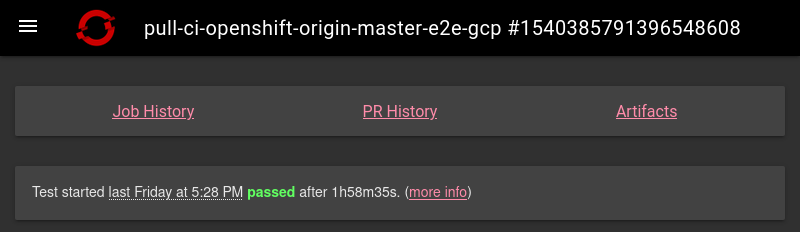
\includegraphics[width=\textwidth]{img/job.png}
        \footnotesize
        \url{https://prow.ci.openshift.org/view/gs/origin-ci-test/pr-logs/pull/27275/pull-ci-openshift-origin-master-e2e-gcp/1540385791396548608}
    \end{center}
    \note{
        From here, it is instructive to examine a typical E2E test, which
        differs quite a bit from the simple container tests we have considered
        so far.  We will look at this test in \texttt{openshift/origin} which
        creates an ephemeral GCP cluster.
    }
\end{frame}

\begin{frame}[fragile]
    \autotitle
    \footnotesize
    \url{https://github.com/openshift/release/blob/master/ci-operator/config/openshift/origin/openshift-origin-master.yaml}
    \normalsize
    \begin{verbatim}
tests:
- as: e2e-gcp
  steps:
    cluster_profile: gcp-openshift-gce-devel-ci-2
    workflow: openshift-e2e-gcp-loki
    \end{verbatim}
    \note{
        This job is generated from this innocent-looking entry in the
        \texttt{ci-operator} configuration file.

        N.b.: take it from someone who has seen all incarnations of Prow job
        definitions we have had, the fact that this test is generated from these
        four lines is a \emph{miracle}.
    }
\end{frame}

\begin{frame}[fragile]
    \autotitle
    \tiny
    \begin{verbatim}
INFO[2022-06-24T17:28:45Z] ci-operator version v20220621-3b245f722
INFO[2022-06-24T17:28:45Z] Loading configuration from https://config.ci.openshift.org for openshift/…
INFO[2022-06-24T17:28:46Z] Resolved source https://github.com/openshift/origin to master@a946e2b9, m…
INFO[2022-06-24T17:28:46Z] Building release previous from a snapshot of ocp/4.10
INFO[2022-06-24T17:28:46Z] Building release initial from a snapshot of ocp/4.11
INFO[2022-06-24T17:28:46Z] Building release latest from a snapshot of ocp/4.11
INFO[2022-06-24T17:28:47Z] Using namespace https://console.build02.ci.openshift.org/k8s/cluster/proj…
INFO[2022-06-24T17:28:47Z] Running [input:root], [input:ocp_builder_rhel-8-golang-1.15-openshift-4.8…
INFO[2022-06-24T17:28:47Z] Tagging ocp/builder:rhel-8-golang-1.15-openshift-4.8 into pipeline:ocp_bu…
INFO[2022-06-24T17:28:47Z] Tagging ocp/builder:rhel-8-golang-1.18-openshift-4.11 into pipeline:ocp_b…
…
INFO[2022-06-24T17:28:48Z] Building src
INFO[2022-06-24T17:32:03Z] Build src succeeded after 3m57s
INFO[2022-06-24T17:32:03Z] Building hello-openshift
INFO[2022-06-24T17:32:03Z] Building tests
INFO[2022-06-24T17:35:23Z] Build hello-openshift succeeded after 3m20s
INFO[2022-06-24T17:35:23Z] Tagging hello-openshift into stable
INFO[2022-06-24T17:42:13Z] Build tests succeeded after 6m48s
INFO[2022-06-24T17:42:13Z] Tagging tests into stable
INFO[2022-06-24T17:42:14Z] Creating release image registry.build02.ci.openshift.org/ci-op-8yq06grj/r…
INFO[2022-06-24T17:43:34Z] Snapshot integration stream into release 4.11.0-0.ci.test-2022-06-24-1742…
INFO[2022-06-24T17:43:34Z] Acquiring leases for test e2e-gcp: [gcp-openshift-gce-devel-ci-2-quota-sl…
INFO[2022-06-24T17:43:34Z] Acquired 1 lease(s) for gcp-openshift-gce-devel-ci-2-quota-slice: [us-cen…
INFO[2022-06-24T17:43:34Z] Running multi-stage test e2e-gcp
INFO[2022-06-24T17:43:34Z] Running multi-stage phase pre
INFO[2022-06-24T17:43:34Z] Running step e2e-gcp-ipi-install-hosted-loki.
…
INFO[2022-06-24T19:27:16Z] Releasing leases for test e2e-gcp
INFO[2022-06-24T19:27:17Z] Ran for 1h58m30s
INFO[2022-06-24T19:27:17Z] Reporting job state 'succeeded'
    \end{verbatim}
    \note{Here is what the output looks like.}
\end{frame}

\begin{frame}
    \autotitle
    \begin{center}
        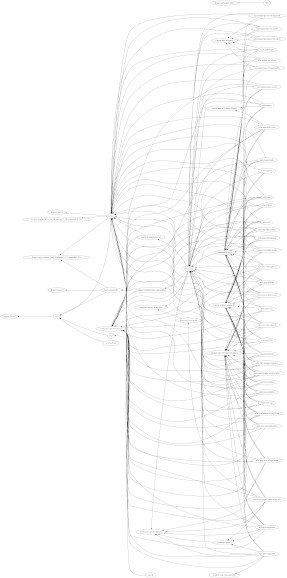
\includegraphics[scale=.35]{img/graph_origin_full.jpg} \\
    \end{center}
    \note{(a reminder that this is what we are dealing with)}
\end{frame}

\begin{frame}
    \autotitle
    \begin{center}
        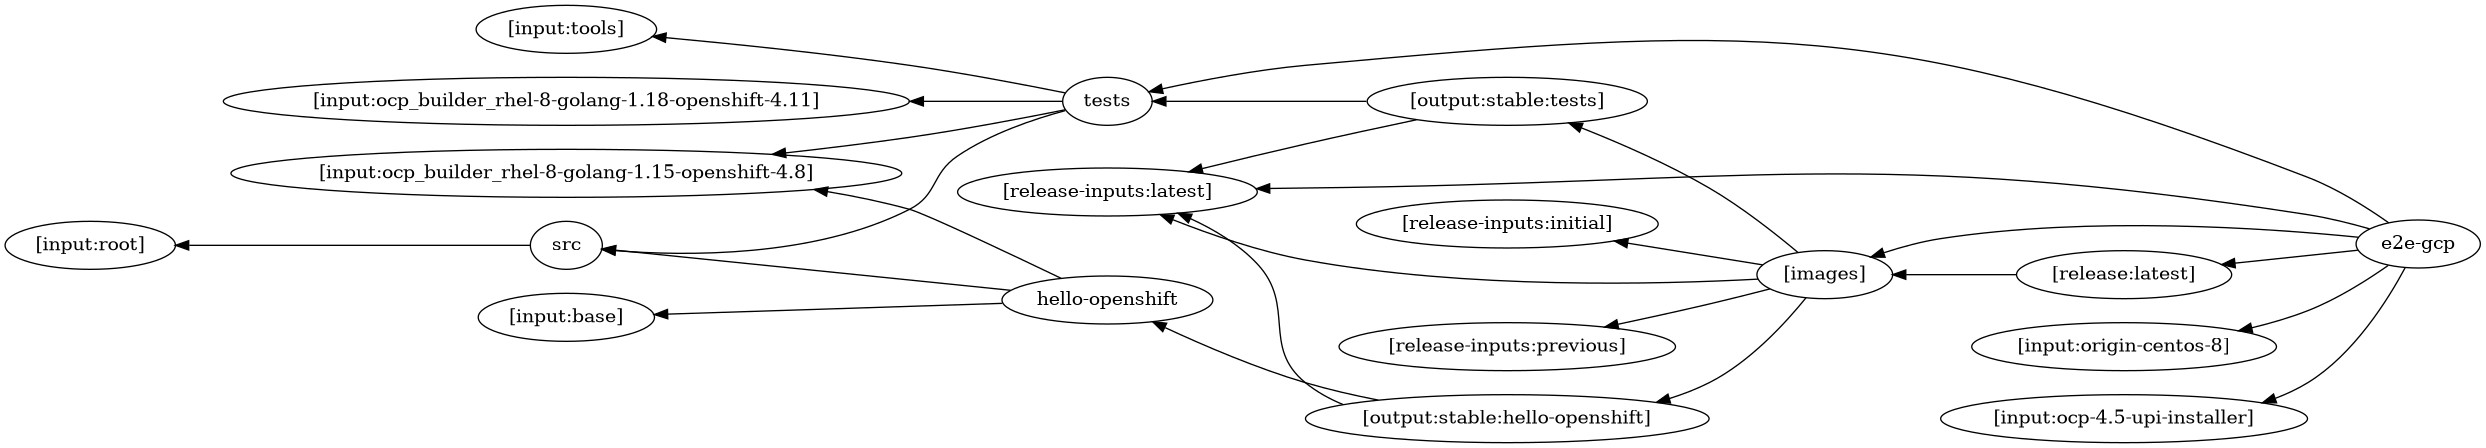
\includegraphics[width=\textwidth]{img/graph_origin_gcp.jpg} \\
    \end{center}
    \note{
        Thankfully, for this particular test, we "only" have to deal with this
        sub-graph.  Let's examine each part.
    }
\end{frame}

\begin{frame}[fragile]
    \autotitle
    \small
    \begin{verbatim}
ci-operator version v20220621-3b245f722
Loading configuration \
    from https://config.ci.openshift.org \
    for openshift/origin@master
Resolved source https://github.com/openshift/origin \
    to master@a946e2b9, merging: \
    #27275 457391d6 @DennisPeriquet
    \end{verbatim}
    \note{We start with the part you are already familiar with.}
\end{frame}

\begin{frame}[fragile]
    \autotitle
    \small
    \begin{verbatim}
Building release previous from a snapshot of ocp/4.10
Building release initial from a snapshot of ocp/4.11
Building release latest from a snapshot of ocp/4.11
    \end{verbatim}
    \footnotesize
    \begin{verbatim}
releases:
  initial:
    integration:
      name: "4.11"
      namespace: ocp
  latest:
    integration:
      include_built_images: true
      name: "4.11"
      namespace: ocp
  previous:
    integration:
      name: "4.10"
      namespace: ocp
    \end{verbatim}
    \note{
        Release images are also root nodes, so they are imported immediately.
        These are all integration streams, which means they come from an
        \texttt{ImageStream} and can simply be copied into the test namespace
        (this is what "snapshot" refers to).
    }
\end{frame}

\begin{frame}
    \autotitle
    \begin{center}
        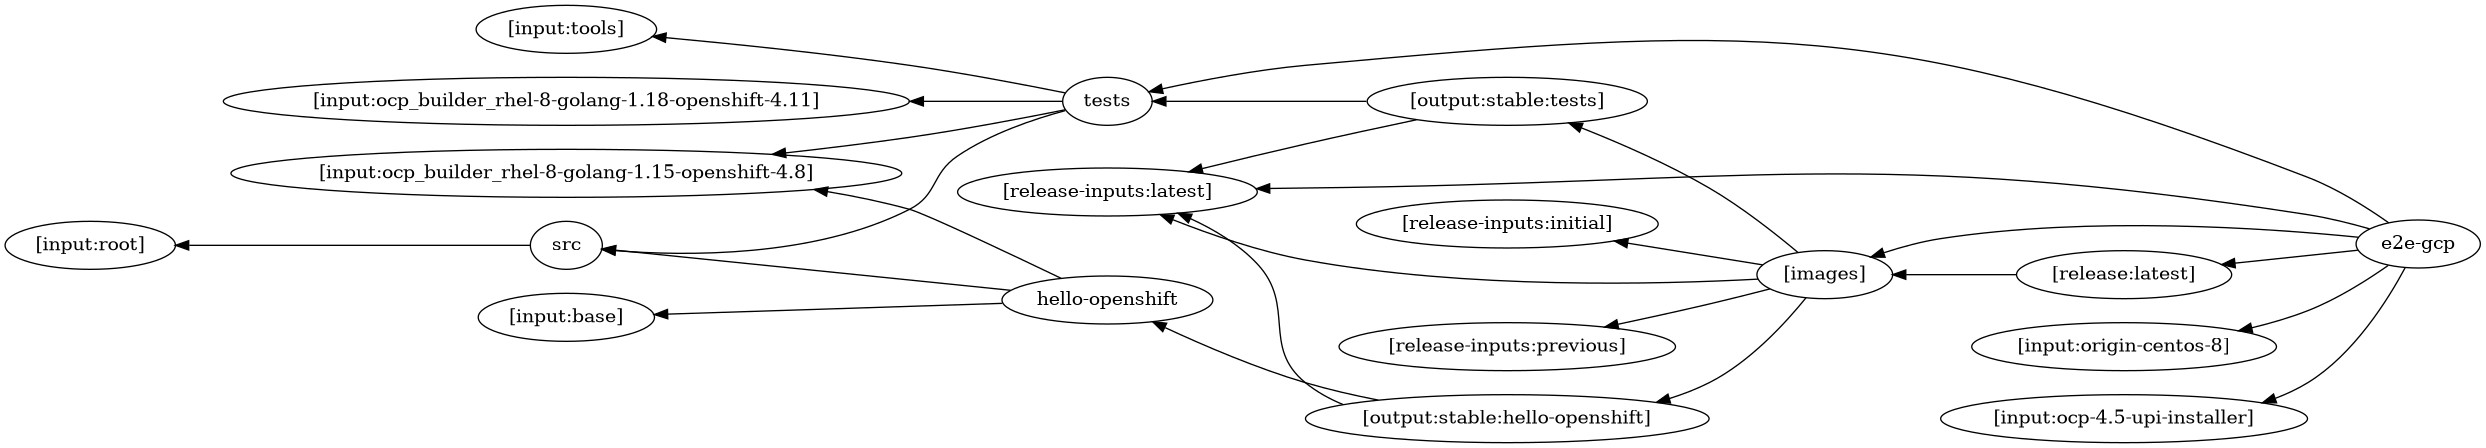
\includegraphics
            [width=\textwidth, clip, trim=900bp 0 700bp 0]
            {img/graph_origin_gcp.jpg}
    \end{center}
    \note{These correspond to the \texttt{[release-inputs:…]} steps here.}
\end{frame}

\begin{frame}[fragile]
    \autotitle
    \footnotesize
    \begin{verbatim}
Using namespace https://console.build02.ci.openshift.org/\
    k8s/cluster/projects/ci-op-8yq06grj
Running [input:root], \
    [input:ocp_builder_rhel-8-golang-1.15-openshift-4.8], \
    [input:ocp_builder_rhel-8-golang-1.18-openshift-4.11], \
    [input:tools], [input:base], [input:origin-centos-8], \
    [input:ocp-4.5-upi-installer], [release-inputs:previous], \
    [release-inputs:initial], [release-inputs:latest], \
    src, tests, hello-openshift, \
    [output:stable:tests], [output:stable:hello-openshift], \
    [images], [release:latest], e2e-gcp
    \end{verbatim}
    \note{
        Here we get assigned a temporary namespace and print the execution
        graph.  Note the same left-to-right order of dependencies, with the
        actual test at the far right of the list.
    }
\end{frame}

\begin{frame}[fragile]
    \autotitle
    \scriptsize
    \begin{verbatim}
Tagging ocp/builder:rhel-8-golang-1.15-openshift-4.8 into \
    pipeline:ocp_builder_rhel-8-golang-1.15-openshift-4.8.
Tagging ocp/builder:rhel-8-golang-1.18-openshift-4.11 into \
    pipeline:ocp_builder_rhel-8-golang-1.18-openshift-4.11.
Tagging openshift/release:rhel-8-release-golang-1.18-openshift-4.11 \
    into pipeline:root.
Tagging origin/centos:8 into pipeline:origin-centos-8.
Tagging ocp/4.11:base into pipeline:base.
Tagging ocp/4.5:upi-installer into pipeline:ocp-4.5-upi-installer.
Tagging ocp/4.11:tools into pipeline:tools.
    \end{verbatim}
    \note{
        The roots of the graph are usually input images, since both the build
        root and base images are depended on for image builds and tests.
    }
\end{frame}

\begin{frame}
    \autotitle
    \begin{center}
        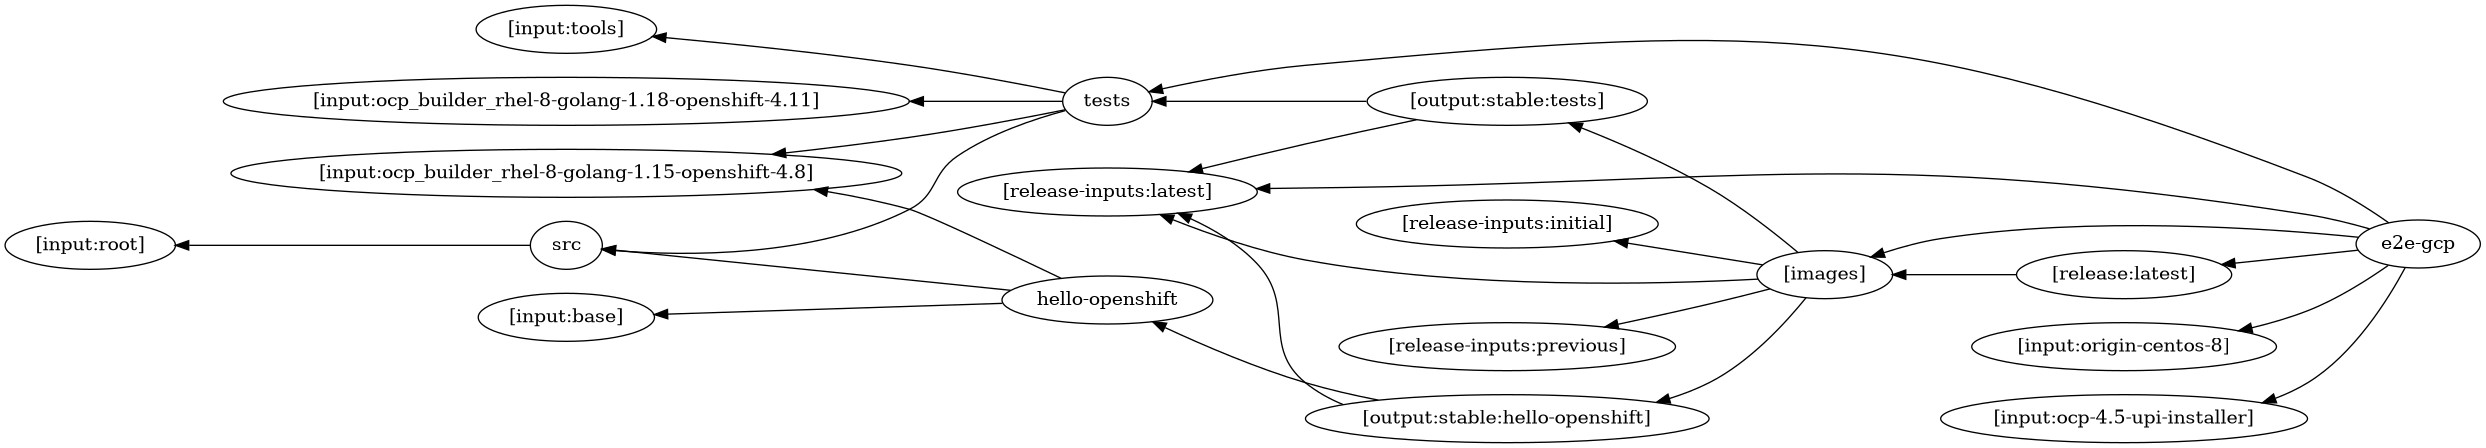
\includegraphics
            [width=\textwidth, clip, trim=0 0 1300bp 0]
            {img/graph_origin_gcp.jpg}
    \end{center}
    \note{
        We see them at the far left side of the graph: they are all in the
        format \texttt{[input:…]}.  Note the dependent image builds.
    }
\end{frame}

\begin{frame}
    \autotitle
    \begin{center}
        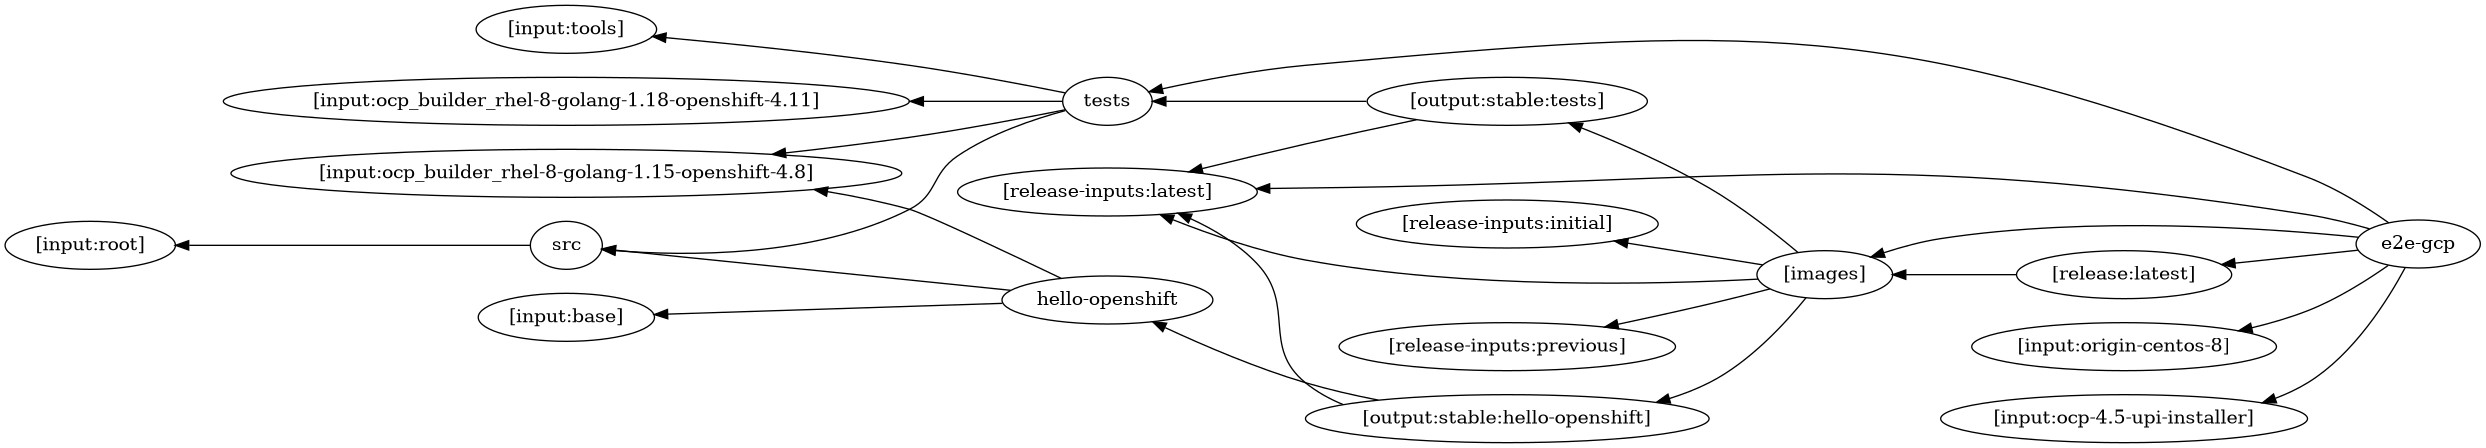
\includegraphics
            [scale=.4, clip, trim=1900bp 0 0 0]
            {img/graph_origin_gcp.jpg}
    \end{center}
    \note{
        And again at the far right for input images depended on by the test
        (more on that later).  These are all independent, so they are imported
        in parallel.
    }
\end{frame}

\begin{frame}[fragile]
    \autotitle
    \footnotesize
    \begin{verbatim}
base_images:
  base: {…}
  ocp_builder_rhel-8-golang-1.15-openshift-4.8: {…}
  ocp_builder_rhel-8-golang-1.18-openshift-4.11: {…}
  tools: {…}
    \end{verbatim}
    \note{
        These images are imported directly using \texttt{base\_images}.
    }
\end{frame}

\begin{frame}[fragile]
    \autotitle
    \begin{verbatim}
build_root:
  from_repository: true
    \end{verbatim}
    \small
    \url{https://github.com/openshift/origin/blob/master/.ci-operator.yaml}
    \normalsize
    \begin{verbatim}
build_root_image:
  name: release
  namespace: openshift
  tag: rhel-8-release-golang-1.18-openshift-4.11
    \end{verbatim}
    \note{
        The \texttt{build\_root} image comes from the repository (you can see
        how these things start to get difficult to track).

        As an aside, when \texttt{from\_repository} is used, we have to make
        sure the Prow job (which executes \texttt{ci-operator}) is configured
        with \texttt{decorate} and does not have \texttt{skip\_cloning}.
        \texttt{ci-operator} will then have access to the the repository code,
        where the \texttt{.ci-operator.yaml} file resides.
    }
\end{frame}

\begin{frame}[fragile]
    \autotitle
    \footnotesize
    \url{https://steps.ci.openshift.org/workflow/openshift-e2e-gcp-loki}
    \small
    \begin{verbatim}
workflow:
  as: openshift-e2e-gcp-loki
  steps:
    allow_best_effort_post_steps: true
    pre:
    - ref: ipi-install-hosted-loki
    - chain: ipi-gcp-pre
    test:
    - ref: openshift-e2e-test
    post:
    - chain: ipi-gcp-post
  documentation: |-
    The Openshift E2E GCP workflow executes the common
    end-to-end test suite on GCP with a default cluster
    configuration with loki as log collector.
    \end{verbatim}
    \note{
        Finding the source of the other images requires us to start looking into
        multi-stage tests.  The \texttt{openshift-e2e-gcp-loki} workflow
        declared in the test can be found in the step registry.  It includes a
        chain called \texttt{ipi-gcp-pre}…
    }
\end{frame}

\begin{frame}[fragile]
    \autotitle
    \url{https://steps.ci.openshift.org/chain/ipi-gcp-pre}
    \begin{verbatim}
chain:
  as: ipi-gcp-pre
  steps:
  - chain: ipi-conf-gcp
  - chain: ipi-install
  documentation: |-
    The IPI setup step contains all steps that
    provision an OpenShift cluster with a default
    configuration on GCP.
    \end{verbatim}
    \note{which includes a chain called \texttt{ipi-conf-gcp}…}
\end{frame}

\begin{frame}[fragile]
    \autotitle
    \url{https://steps.ci.openshift.org/chain/ipi-conf-gcp}
    \begin{verbatim}
chain:
  as: ipi-conf-gcp
  steps:
  - ref: ipi-conf
  - ref: ipi-conf-gcp
  - ref: ipi-install-monitoringpvc
  documentation: >-
    This chain generates an install-config.yaml
    file configured to run clusters in the GCP CI
    project.
    The GCP specific configs are added to
    the file generated by the ipi-conf steps.
    This resulting file is stored in the shared
    directory for future consumption.
    \end{verbatim}
    \note{
        which includes steps called \texttt{ipi-conf} and \texttt{ipi-conf-gcp}…
    }
\end{frame}

\begin{frame}[fragile]
    \autotitle
    \small
    \url{https://steps.ci.openshift.org/reference/ipi-conf}
    \url{https://steps.ci.openshift.org/reference/ipi-conf-gcp}
    \normalsize
    \begin{verbatim}
ref:
  as: ipi-conf
  from_image:
   namespace: origin
   name: centos
   tag: '8'
    \end{verbatim}
    ($\texttt{from\_image} \approx \texttt{base\_images} + \texttt{from}$)
    \note{
        and here we finally find our \texttt{centos:8} image.
        \texttt{from\_image} entries for all steps are collected and added to
        the input images in \texttt{base\_images}.
    }
\end{frame}

\begin{frame}[fragile]
    \autotitle
    \footnotesize
    \url{https://steps.ci.openshift.org/reference/gather-gcp-console}
    \normalsize
    \begin{verbatim}
ref:
  as: gather-gcp-console
  optional_on_success: true
  from_image:
    namespace: ocp
    name: "4.5"
    tag: upi-installer
    …
    \end{verbatim}
    \note{
        Similarly, \texttt{upi-installer} can be found in the
        \texttt{gather-gcp-console} step.
    }
\end{frame}

\begin{frame}[fragile]
    \autotitle
    \small
    \begin{verbatim}
Building src
Build src succeeded after 3m57s
Building hello-openshift
Building tests
Build hello-openshift succeeded after 3m20s
Tagging hello-openshift into stable
Build tests succeeded after 6m48s
Tagging tests into stable
    \end{verbatim}
    \note{
        After the required images are imported, image builds can be started.
    }
\end{frame}

\begin{frame}
    \autotitle
    \begin{center}
        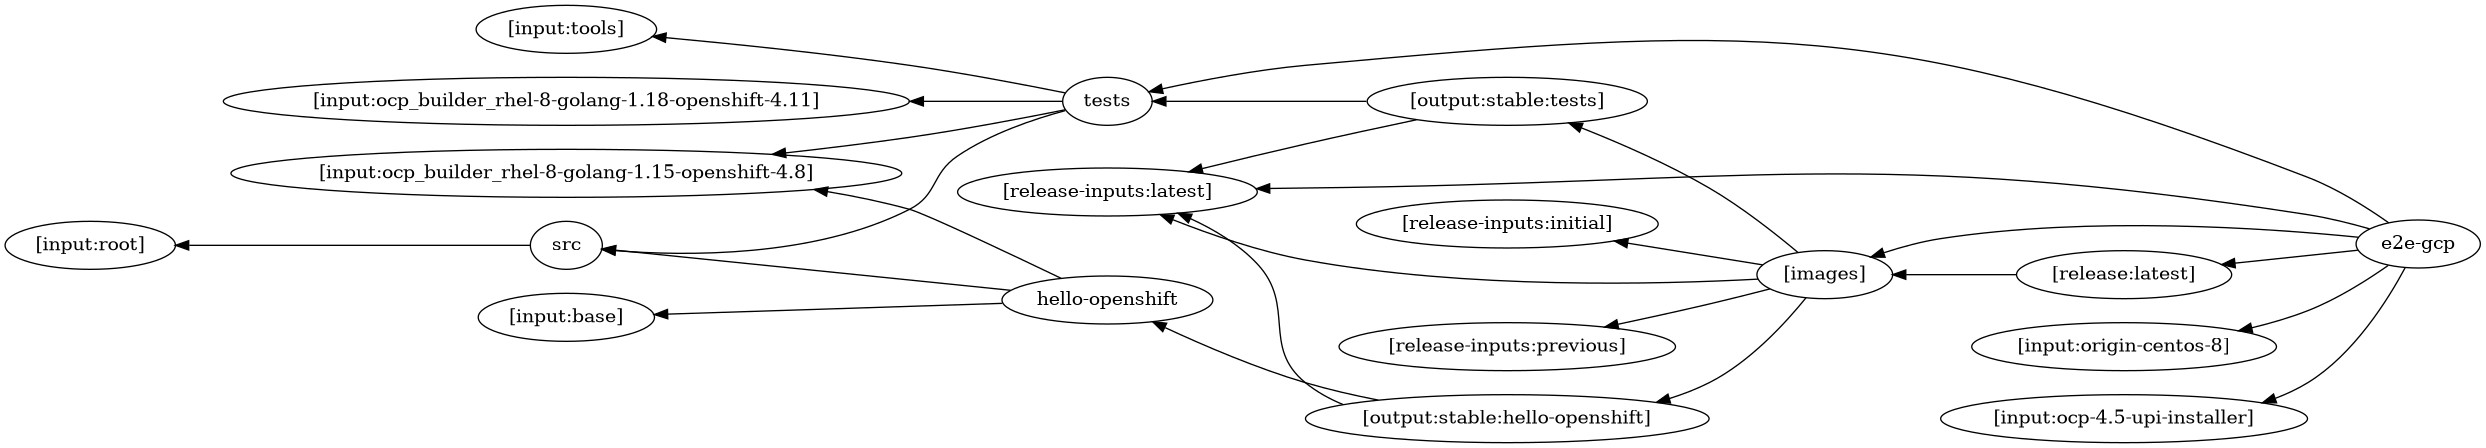
\includegraphics
            [width=\textwidth, clip, trim=450bp 0 1200bp 0]
            {img/graph_origin_gcp.jpg}
    \end{center}
    \note{
        \texttt{src} is built first, since it is a requirement for the other
        two, which are then built in parallel.
    }
\end{frame}

\begin{frame}[fragile]
    \autotitle
    \small
    \begin{verbatim}
Build hello-openshift succeeded after 3m20s
Tagging hello-openshift into stable
Build tests succeeded after 6m48s
Tagging tests into stable
    \end{verbatim}
    \note{
        Each image that is built is also tagged into the \texttt{stable}
        \texttt{ImageStream}.
    }
\end{frame}

\begin{frame}
    \autotitle
    \begin{center}
        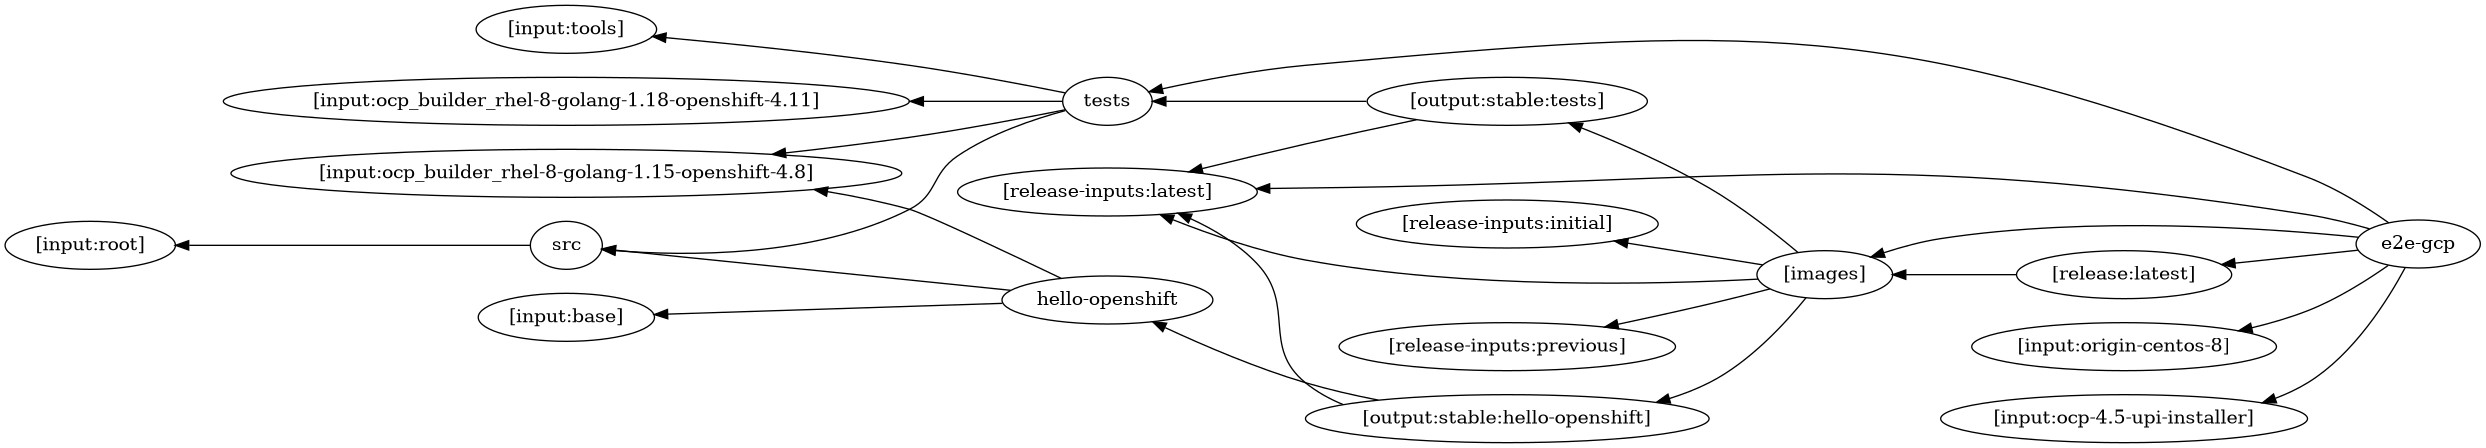
\includegraphics
            [width=\textwidth, clip, trim=950bp 0 550bp 0]
            {img/graph_origin_gcp.jpg}
    \end{center}
    \note{These are done by the steps in the format \texttt{[output:…]}.}
\end{frame}

\begin{frame}
    \autotitle
    \begin{center}
        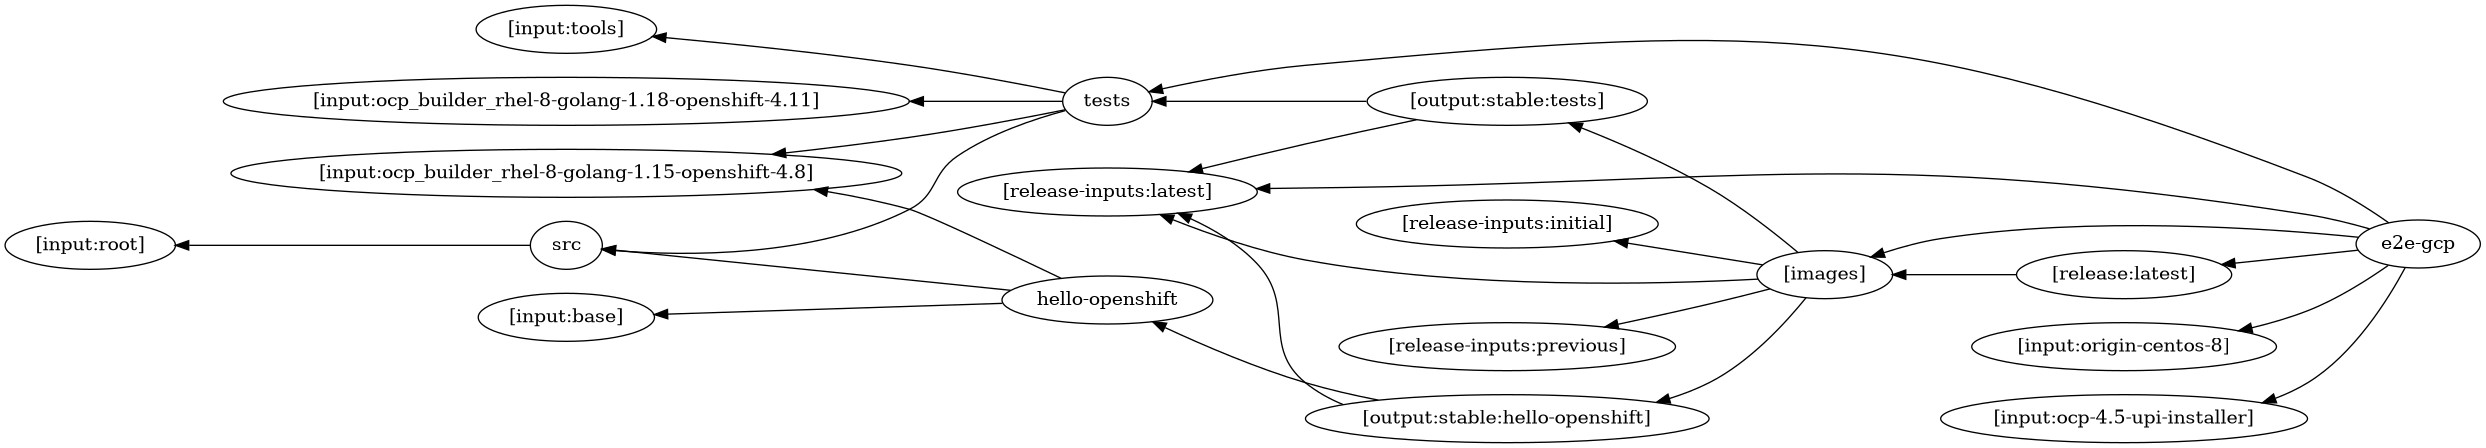
\includegraphics
            [width=\textwidth, clip, trim=950bp 0 0 0]
            {img/graph_origin_gcp.jpg}
    \end{center}
    \note{
        This is difficult to capture since it is right in the middle of the
        graph, but notice the \texttt{[images]} step acting as a synchronization
        point between image build / release image imports and the release
        payload generation / test.

        That is all it does: it is a synthetic step created purely to guarantee
        these operations are done in the proper order.
    }
\end{frame}

\begin{frame}[fragile]
    \autotitle
    \footnotesize
    \url{https://github.com/openshift/release/blob/master/ci-operator/jobs/openshift/origin/openshift-origin-master-postsubmits.yaml}
    (simplified)
    \normalsize
    \begin{verbatim}
name: branch-ci-openshift-origin-master-images
spec:
  containers:
  - args:
    - --target=[images]
    - --promote
    command:
    - ci-operator
    \end{verbatim}
    \note{
        It can also be used as a target, such as we do in the \texttt{*-images}
        post-submit jobs.
    }
\end{frame}

\begin{frame}[fragile]
    \autotitle
    \footnotesize
    \begin{verbatim}
Creating release image registry.build02.ci.openshift.org/\
    ci-op-8yq06grj/release:latest.
Snapshot integration stream into release \
    4.11.0-0.ci.test-2022-06-24-174214-ci-op-8yq06grj-latest \
    to tag release:latest
    \end{verbatim}
    \note{
        We now create the release payload from the \texttt{stable}
        \texttt{ImageStream}.  The latter contains the initial images imported
        from the integration stream, along with the images just built from the
        input source code (recall they were tagged into \texttt{stable} after
        they were built).

        By overlaying the new tags on top of the existing streams, we get a
        release payload where the repository images are overwritten by the ones
        which were just built from the input source code.
    }
\end{frame}

\begin{frame}[fragile]
    \autotitle
    \begin{verbatim}
releases:
  latest:
    integration:
      include_built_images: true
      name: "4.11"
      namespace: ocp
    \end{verbatim}
\end{frame}

\begin{frame}
    \autotitle
    \begin{center}
        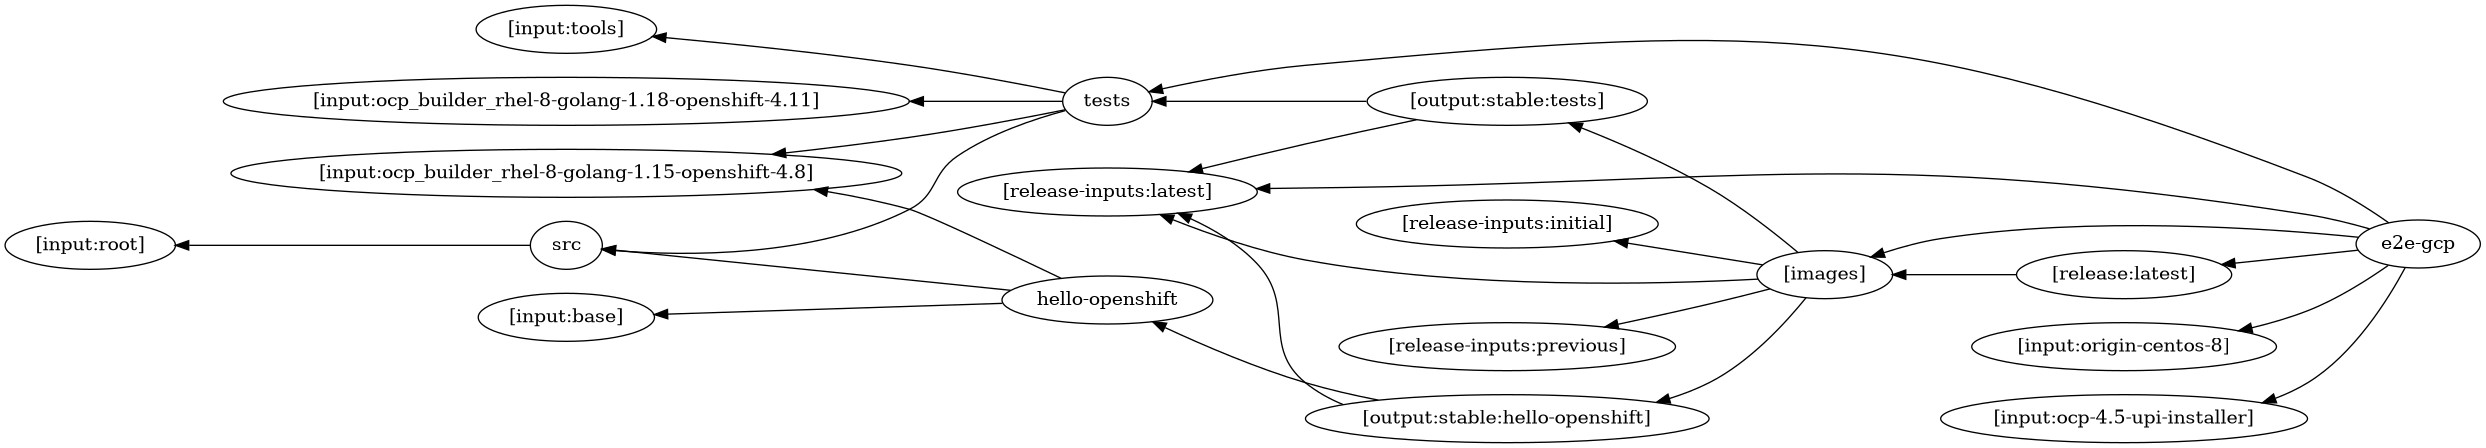
\includegraphics
            [width=\textwidth, clip, trim=1600bp 0 100bp 0]
            {img/graph_origin_gcp.jpg}
    \end{center}
    \note{
        This is what the \texttt{[release:latest]} job does.  The dependency on
        that step by the E2E test makes the resulting image available to the
        latter to be used by the installer to create the ephemeral cluster.
    }
\end{frame}

\begin{frame}[fragile]
    \autotitle
    \footnotesize
    \begin{verbatim}
Acquiring leases for test e2e-gcp: \
    [gcp-openshift-gce-devel-ci-2-quota-slice]
Acquired 1 lease(s) for \
    gcp-openshift-gce-devel-ci-2-quota-slice: \
    [us-central1--gcp-openshift-gce-devel-ci-2-quota-slice-08]
    \end{verbatim}
    \note{
        We are finally at the beginning of the test execution now.  Because it
        is an E2E test (approximated by "it declares a cluster profile"),
        \texttt{ci-operator} will contact the leasing server (i.e.
        \href{https://github.com/kubernetes-sigs/boskos.git}{Boskos}) to acquire
        a lease for the ephemeral cluster.
    }
\end{frame}

\begin{frame}[fragile]
    \autotitle
    \url{https://github.com/openshift/ci-tools/blob/master/pkg/api/types.go}
    (heavily abbreviated)
    \footnotesize
    \begin{verbatim}
type ClusterProfile string

const ClusterProfileGCP2 ClusterProfile =
    "gcp-openshift-gce-devel-ci-2"

func (p ClusterProfile) LeaseType() string {
    switch p {
    case ClusterProfileGCP2:
        return "gcp-openshift-gce-devel-ci-2-quota-slice"
    }
}
    \end{verbatim}
    \note{
        Each cluster profile (a string) is registered in \texttt{ci-tools} and
        associated with a resource type.
    }
\end{frame}

\begin{frame}[fragile]
    \autotitle
    \footnotesize
    \begin{verbatim}
Running multi-stage test e2e-gcp
Running multi-stage phase pre
Running step e2e-gcp-ipi-install-hosted-loki.
Step e2e-gcp-ipi-install-hosted-loki succeeded after 20s.
Running step e2e-gcp-ipi-conf.
Step e2e-gcp-ipi-conf succeeded after 20s.
…
Running multi-stage phase test
Running step e2e-gcp-openshift-e2e-test.
Step e2e-gcp-openshift-e2e-test succeeded after 55m0s.
Step phase test succeeded after 55m0s.
Running multi-stage phase post
Running step e2e-gcp-gather-gcp-console.
Step e2e-gcp-gather-gcp-console succeeded after 50s.
…
Step phase post succeeded after 16m40s.
    \end{verbatim}
\end{frame}

\begin{frame}[fragile]
    \autotitle
    \begin{verbatim}
Releasing leases for test e2e-gcp
Ran for 1h58m30s
Reporting job state 'succeeded'
    \end{verbatim}
\end{frame}

\subsection{Etc.}
\begin{frame}
    \autotitle
    \begin{multicols}{2}
        \begin{itemize}
            \item build clusters
            \item \href
                {https://github.com/openshift/ci-ns-ttl-controller}
                {\texttt{ci-ns-ttl-controller}}
            \item image distribution
            \item types of \texttt{releases}
            \item (\textit{init}) containers
            \item test types
                \begin{itemize}
                    \item container
                    \item template
                    \item multi-stage
                \end{itemize}
            \item artifacts
            \item image promotion
        \end{itemize}
    \end{multicols}
\end{frame}


\begin{frame}
    \usebeamertemplate{end page}
\end{frame}

\end{document}
